\documentclass{article}
\usepackage[utf8]{inputenc}
\usepackage{amsmath,amsthm}
\usepackage[inline,shortlabels]{enumitem}
\usepackage{fancyvrb}
\usepackage{graphicx}
\usepackage{hyperref}
\usepackage{subcaption}
\usepackage{tikz}

\newtheorem{thm}{Theorem}[section]
\theoremstyle{definition}
\newtheorem{Def}{Definition}[section]
\theoremstyle{remark}
\newtheorem{Rmk}{Remark}[section]
\newtheorem*{Nt}{Note}

\title{Latex Certificate Course Instructions}
\author{Jacob Antony}
\date{\today}

\begin{document}

\maketitle

\section{figure Environment}
	The \texttt{figure} environment is used for adding figures to your document. The \texttt{figure} environments can have captions. You may also generate a list of figures using \texttt{\textbackslash listoffigures} command.

\subsection{includegraphics Command}
	The \texttt{figure} environments are supposed to contain images that you draw using \LaTeX{} or that you already have in your computer.
	
	You can add images on your computer to the document using \texttt{\textbackslash includegraphics} command. This command takes the image address as argument and image dimensions and effects as optional arguments. And it does not require a \texttt{figure} environment.

\begin{figure}[h]
\centering
\begin{minipage}{0.45\textwidth}
\begin{Verbatim}[numbers = left]
\usepackage{graphicx}
...
\begin{document}
...
\begin{figure}
\centering

\includegraphics{flower.jpg}
\caption{Flower}
\end{figure}
\end{Verbatim}
\end{minipage}
%\begin{subfigure}{0.45\textwidth}
\begin{minipage}{0.45\textwidth}
\centering

\includegraphics[scale=0.05]{flower.jpg}
\caption{Flower}
\end{minipage}
\caption{figure Environment}
\label{fig:figure}
\end{figure}

\subsection{Drawing using Tikz}
	The \texttt{tikz} package is user-friendly syntax layer for the \texttt{pgf} package. The current version of \texttt{pgf} package is 3.1.8b. And is maintained by the PGF-Tikz team. The \texttt{pgf} package documentation is available at \href{https://ctan.org/pkg/pgf}{CTAN} and \href{https://github.com/pgf-tikz/pgf}{Github}.

	\LaTeX{} allows you to create vector images using \texttt{Tikz} package. The \texttt{tikzpicture} enviroment is used and it supports \texttt{\textbackslash draw} commmand which draws a path. 

\begin{figure}[h]
\centering
\begin{minipage}{0.45\textwidth}
\begin{Verbatim}[numbers = left]
\usepackage{tikz}
...
\begin{document}
...
\begin{figure}
\centering
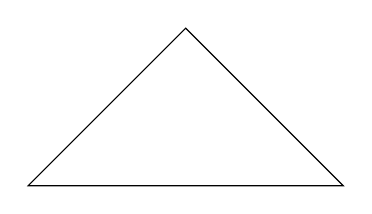
\begin{tikzpicture}
\draw (0,0) -- (2,2) %
-- (4,0) -- cycle;
\end{tikzpicture}
\caption{Triangle}
\label{fig:tikz}
\end{figure}
\end{Verbatim}
\end{minipage}
\begin{minipage}{0.45\textwidth}
\centering
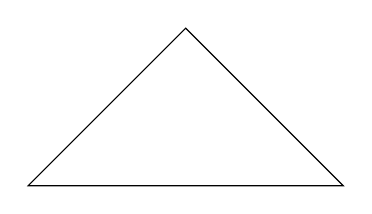
\begin{tikzpicture}
\draw (0,0)--(2,2)%
--(4,0)--cycle;
\end{tikzpicture}
\caption{Triangle}
\end{minipage} 
\caption{Drawing using Tikz}
\label{fig:tikz}
\end{figure}

	In Figure \ref{fig:tikz} at line 12, an anchor named \texttt{fig:tikz} is created. The purpose of anchors will be discussed in section \ref{sec:reference}.

\subsubsection{Tikz Coordinate Systems}
	In Figure \ref{fig:tikz} at line 8, the ordered pairs $(0,0)$, $(2,2)$ and $(4,0)$ represents coordinates in the cartesian coordinate system. You may also write \texttt{(2:45)} which represent $2 \angle 45$ in the polar coordinate system. Tikz also supports relative coordinates. \texttt{++(2,2)} represents $2$ units to the right and $2$ units to the top. Similarly, \texttt{++(2:45)} represents $2$ units at $45$ degrees.

	In Tikz, \texttt{\textbackslash coordinate} command is used to name coordinates. Then you can use those names to draw paths. For example, \texttt{\textbackslash coordinate (A) at (0,0);} names the coordinate $(0,0)$ as \texttt{A}.

\subsubsection{Tikz Path Commands}
	Tikz \texttt{\textbackslash path} command is used to define paths. This path is not visible if not mentioned explicitly. Also paths can be assigned names. The \texttt{\textbackslash path} command has the following variants,
\begin{description}
	\item[\texttt{\textbackslash draw}] draws the path
	\item[\texttt{\textbackslash clip}] crops the image inside path
	\item[\texttt{\textbackslash fill}] fill the interior of the path
	\item[\texttt{\textbackslash shade}] shades the interior of the path with a gradient
	\item[\texttt{\textbackslash shadedraw}] shades and draws the path
\end{description}

%\subsubsection{Tikz Path Extension Operations}
%	Tikz supports \texttt{--}, \texttt{to}, \texttt{controls}, \texttt{and}, \texttt{circle}, \texttt{ellipse}, \texttt{arc}, \texttt{rectangle}, \texttt{grid}, \texttt{plot}, \texttt{cycle} as path extension operations.

\subsubsection{Tikz Nodes}
	Tikz allows you add draw an image part by part. The \texttt{\textbackslash node} command is used to draw a part of the image. This part could be just a label or a complex sub-image.

%scope, shift, loops, 

\section{table Environment}
	The \texttt{table} environment is used for adding tables to your document. The \texttt{table} environments can have captions. You may also generate a list of tables using \texttt{\textbackslash listoftables} command.

\subsection{tabular Environment}
	The \texttt{tabular} environment is used for creating tabular data. This environment uses \& to separate columns and \textbackslash{}\textbackslash{} to separate rows. The \texttt{\textbackslash hline} and \texttt{\textbackslash cline} commands are used to draw horizontal lines. The second argument of the \texttt{\textbackslash begin} command is used for drawing vertical lines and aligning data in each column.

\begin{table}[h]
\centering
\begin{subfigure}{0.45\textwidth}
\begin{Verbatim}[numbers = left]
\begin{table}
\begin{tabular}{|c||l|}\hline
No. & Environments \\ \hline
1 & tabular \\ \hline
2 & equation \\ \hline
3 & matrix \\ \hline
\end{tabular}
\caption{Environments}
\label{tb:table}
\end{table}
\end{Verbatim}
\end{subfigure}
\begin{minipage}{0.45\textwidth} 
\centering
\begin{tabular}{|c||l|} \hline
 No. & Environments \\ \hline
1 & tabular \\ \hline
2 & equation \\ \hline
3 & matrix \\ \hline
\end{tabular}
\caption{Environments}
\label{tb:table}
\end{minipage}
\caption{table Environment}
\label{tb:tableEnvironment}
\end{table}

\section{Cross Reference} \label{sec:reference}
	\LaTeX{} has a mechanism to refer different elements of the same document. You can refer to equations, sections, tables and figures. The \texttt{\textbackslash label} command is used to create an anchor of reference. And \texttt{\textbackslash ref} command is used to refer to such an anchor. Also \texttt{\textbackslash pageref} command is used to refer to the page number of that anchor.
	
	You can have forward references as \LaTeX{} creates/updates anchors in the associated \texttt{aux} file. And updates the references using the existing labels in the \texttt{aux} file. You might have to compile twice to update labels which are newly introduced.

\subsection{Adding Anchors}
	The \texttt{\textbackslash label} command is used to create anchors.
	
	In Figure \ref{fig:tikz} at line 12, an anchor \texttt{fig:tikz} is created. And in Table \ref{tb:table} at line 9, another anchor \texttt{tb:table} is created. These anchor may be referenced using the command \texttt{\textbackslash ref}. 
	
	For example, \texttt{\textbackslash ref\{fig:tikz\}} gives \ref{fig:tikz}. And, \texttt{\textbackslash pageref\{tb:table\}} gives \pageref{tb:table}. The anchor \texttt{fig:tikz} is the figure numbered \ref{fig:tikz} and \texttt{tb:table} is the table on page \pageref{tb:table}. These numbers are automatically updated by \LaTeX{}.

\paragraph{Warning :}
	The \texttt{figure} and \texttt{table} numbers are updated only if they have a caption. Thus, \texttt{\textbackslash label} command won't work in \texttt{figure} and \texttt{table} environments if it is not used after the \texttt{\textbackslash caption} command.

\subsection{Associated Files}
	There are many associated files created and managed by \LaTeX{} for generating your document. The files with \texttt{tex} extension are \LaTeX{} source files where you write your \LaTeX{} file for document creation. The \texttt{pdf} extension is used by the PDF files generated by \LaTeX{}. 

	We can tell the purpose of each associated file from its file extension. The following are a few important file extensions,
\begin{description}
	\item[aux] Auxiliary Data for toc, reference, index, bibliography, \dots
	\item[log] Compilation Log --- Errors and Warnings
	\item[toc] Table of Contents
	\item[lof] List of Figures
	\item[lot] List of Tables
\end{description}

An ellaborate list of file extensions for different purposes, is available at \href{https://tex.stackexchange.com/questions/7770/file-extensions-related-to-latex-etc}{Tex StackExchange}.

\end{document}
